\chapter{Results}
\label{sec:Results}

In this section the results of the cross-section calculations are presented. The results of the integral and differential cross-sections (as defined in Section~\ref{sec:ZeeCrossSec}) are shown together with uncertainties and theoretical predictions. There are two main types of the uncertainties: statistical and systematical, and whereas the statistical uncertainties are trivial to calculate, and depend only on the amount of the data in any given bin, the sources for the systematical uncertainties are much more numerous. The sources for the different systematical uncertainties are listed in Tab.~\ref{tab:Zee_unc_list_peak} for peak mass region and in Tab.~\ref{tab:Zee_unc_list_high} for high mass region. The efficiency uncertainties were described in the Section~\ref{sec:Efficiency}, the resolution and scale were described in Section~\ref{sec:Reconstruction}, the background was described in Section~\ref{sec:Bkg}, and the rest are the theory uncertainties. The systematic uncertainties are also shown at Figure~\ref{fig:Zee_unc}. Note, that on the image the different uncertainties are just stacked one on top of another, so the total amount of uncertainty shown on the plot in every given bin won't be the same as the resulting uncertainty for that bin, which would require the quadratic sum. From the plots it can be easily seen, that for the peak mass region the uncertainties are largely dominated by the identification efficiency for the forward electron, while in the high mass region the main contributors is the forward electron resolution.

\begin{table}
\centering
\begin{tabular}{l r p{0.7cm}p{0.7cm}p{0.7cm}p{0.7cm}p{0.7cm}p{0.7cm}p{0.7cm}p{0.7cm}l}
\hline \hline
\multirow{2}{*}{$|\eta|$ bin boundary} & low  & 1.20 & 1.40 & 1.60 & 1.80 & 2.00 & 2.20 & 2.40 & 2.80 & 3.20 \\
                                       & high & 1.40 & 1.60 & 1.80 & 2.00 & 2.20 & 2.40 & 2.80 & 3.20 & 3.60  \\
\hline
\multicolumn{2}{l}{Trigger efficiency}            & 0.159 & 0.072 & 0.067 & 0.064 & 0.070 & 0.068 & 0.089 & 0.115 & 0.220 \\
\multicolumn{2}{l}{Recon. efficiency}             & 0.499 & 0.370 & 0.340 & 0.251 & 0.180 & 0.122 & 0.093 & 0.149 & 0.307 \\
\multicolumn{2}{l}{Id. efficiency}                & 0.258 & 0.223 & 0.210 & 0.166 & 0.157 & 0.133 & 0.164 & 0.216 & 0.436 \\
\multicolumn{2}{l}{Id.Fwd efficiency}             & 3.215 & 2.898 & 2.641 & 2.450 & 2.070 & 1.840 & 1.634 & 5.443 & 6.991 \\
\multicolumn{2}{l}{Iso. efficiency}               & 0.090 & 0.082 & 0.078 & 0.091 & 0.064 & 0.077 & 0.067 & 0.067 & 0.179 \\
\multicolumn{2}{l}{Electron resolution}           & 0.073 & 0.029 & 0.046 & 0.008 & 0.051 & 0.072 & 0.023 & 0.010 & 0.117 \\
\multicolumn{2}{l}{Fwd Electron resolution}       & 0.984 & 0.696 & 0.513 & 1.727 & 2.632 & 1.883 & 3.002 & 0.451 & 0.353 \\
\multicolumn{2}{l}{Electron scale}                & 0.438 & 0.277 & 0.186 & 0.212 & 0.255 & 0.154 & 0.114 & 0.097 & 0.247 \\
\multicolumn{2}{l}{Fwd Electron scale}            & 0.410 & 0.243 & 0.124 & 0.042 & 0.161 & 0.096 & 0.156 & 0.432 & 2.114 \\
\multicolumn{2}{l}{Matrix element}                & 0.138 & 0.138 & 0.138 & 0.138 & 0.138 & 0.138 & 0.138 & 0.138 & 0.138 \\
\multicolumn{2}{l}{PS and hadronization}          & 0.522 & 0.522 & 0.522 & 0.522 & 0.522 & 0.521 & 0.521 & 0.521 & 0.521 \\
\multicolumn{2}{l}{PDF}                           & 0.124 & 0.057 & 0.031 & 0.015 & 0.015 & 0.010 & 0.007 & 0.021 & 0.057 \\
\multicolumn{2}{l}{EW Bkg}                        & 0.386 & 0.325 & 0.197 & 0.163 & 0.156 & 0.132 & 0.120 & 0.064 & 0.029 \\
\multicolumn{2}{l}{QCD Bkg}                       & 0.228 & 0.174 & 0.177 & 0.248 & 0.220 & 0.083 & 0.187 & 0.093 & 0.289 \\
\hline
\multicolumn{2}{l}{Tot. Syst. Uncertainty}        & 3.540 & 3.107 & 2.797 & 3.084 & 3.426 & 2.707 & 3.480 & 5.515 & 7.368 \\
\hline
\multicolumn{2}{l}{Stat. Uncertainty (MC)}        & 0.635 & 0.353 & 0.207 & 0.206 & 0.186 & 0.175 & 0.126 & 0.199 & 0.453 \\
\multicolumn{2}{l}{Stat. Uncertainty}             & 1.763 & 1.019 & 0.730 & 0.595 & 0.580 & 0.499 & 0.339 & 0.494 & 1.227 \\
\hline \hline
\end{tabular}
\caption{The list of the uncertainties in percent for peak mass region.}
\label{tab:Zee_unc_list_peak}
\end{table}

\begin{table}
\centering
\begin{tabular}{l r r r r r r r}
\hline \hline
 \multirow{2}{*}{$|\eta|$ bin boundary} & low  & \multicolumn{1}{l}{1.20} & \multicolumn{1}{l}{1.60} & \multicolumn{1}{l}{2.00}
                                               & \multicolumn{1}{l}{2.40} & \multicolumn{1}{l}{2.80} & \multicolumn{1}{l}{3.20}  \\
                                        & high & 1.60  & 2.00  & 2.40  & 2.80  & 3.20  & 3.60  \\
\hline
\multicolumn{2}{l}{Trigger efficiency}            & 0.067 & 0.037 & 0.058 & 0.109 & 0.139 & 0.191  \\
\multicolumn{2}{l}{Recon. efficiency}             & 0.195 & 0.158 & 0.147 & 0.142 & 0.137 & 0.135  \\
\multicolumn{2}{l}{Id. efficiency}                & 0.132 & 0.113 & 0.170 & 0.246 & 0.256 & 0.243  \\
\multicolumn{2}{l}{Id.Fwd efficiency}             & 2.463 & 1.919 & 1.517 & 1.955 & 5.330 & 7.069  \\
\multicolumn{2}{l}{Iso. efficiency}               & 0.046 & 0.053 & 0.080 & 0.096 & 0.078 & 0.079  \\
\multicolumn{2}{l}{Electron resolution}           & 0.459 & 0.714 & 0.672 & 1.254 & 1.102 & 0.753  \\
\multicolumn{2}{l}{Fwd Electron resolution}       & 2.357 & 5.231 & 12.303 & 20.601 & 14.154 & 1.554  \\
\multicolumn{2}{l}{Electron scale}                & 0.302 & 0.354 & 0.717 & 0.592 & 0.609 & 1.607  \\
\multicolumn{2}{l}{Fwd Electron scale}            & 1.470 & 1.884 & 2.252 & 2.086 & 2.497 & 2.566  \\
\multicolumn{2}{l}{Matrix element}                & 0.606 & 0.568 & 0.429 & 0.494 & 0.488 & 0.565  \\
\multicolumn{2}{l}{PS and hadronization}          & 1.480 & 1.385 & 1.048 & 1.208 & 1.195 & 1.397  \\
\multicolumn{2}{l}{PDF}                           & 0.162 & 0.081 & 0.110 & 0.074 & 0.099 & 0.471  \\
\multicolumn{2}{l}{EW Bkg}                        & 8.332 & 6.544 & 2.880 & 2.144 & 1.184 & 0.000  \\
\multicolumn{2}{l}{QCD Bkg}                       & 5.904 & 5.575 & 5.417 & 3.043 & 1.828 & 10.225  \\
\hline
\multicolumn{2}{l}{Tot. Syst. Uncertainty}        & 11.044 & 10.576 & 14.109 & 21.221 & 15.594 & 13.012 \\
\hline
\multicolumn{2}{l}{Stat. Uncertainty (MC)}        & 1.619 & 1.156 & 0.981 & 0.930 & 1.716 & 3.892  \\
\multicolumn{2}{l}{Stat. Uncertainty}             & 6.845 & 5.213 & 4.023 & 3.886 & 5.291 & 14.533  \\
\hline \hline
\end{tabular}
\caption{The list of the uncertainties in percent for high mass region.}
\label{tab:Zee_unc_list_high}
\end{table}

\begin{figure}
\center{
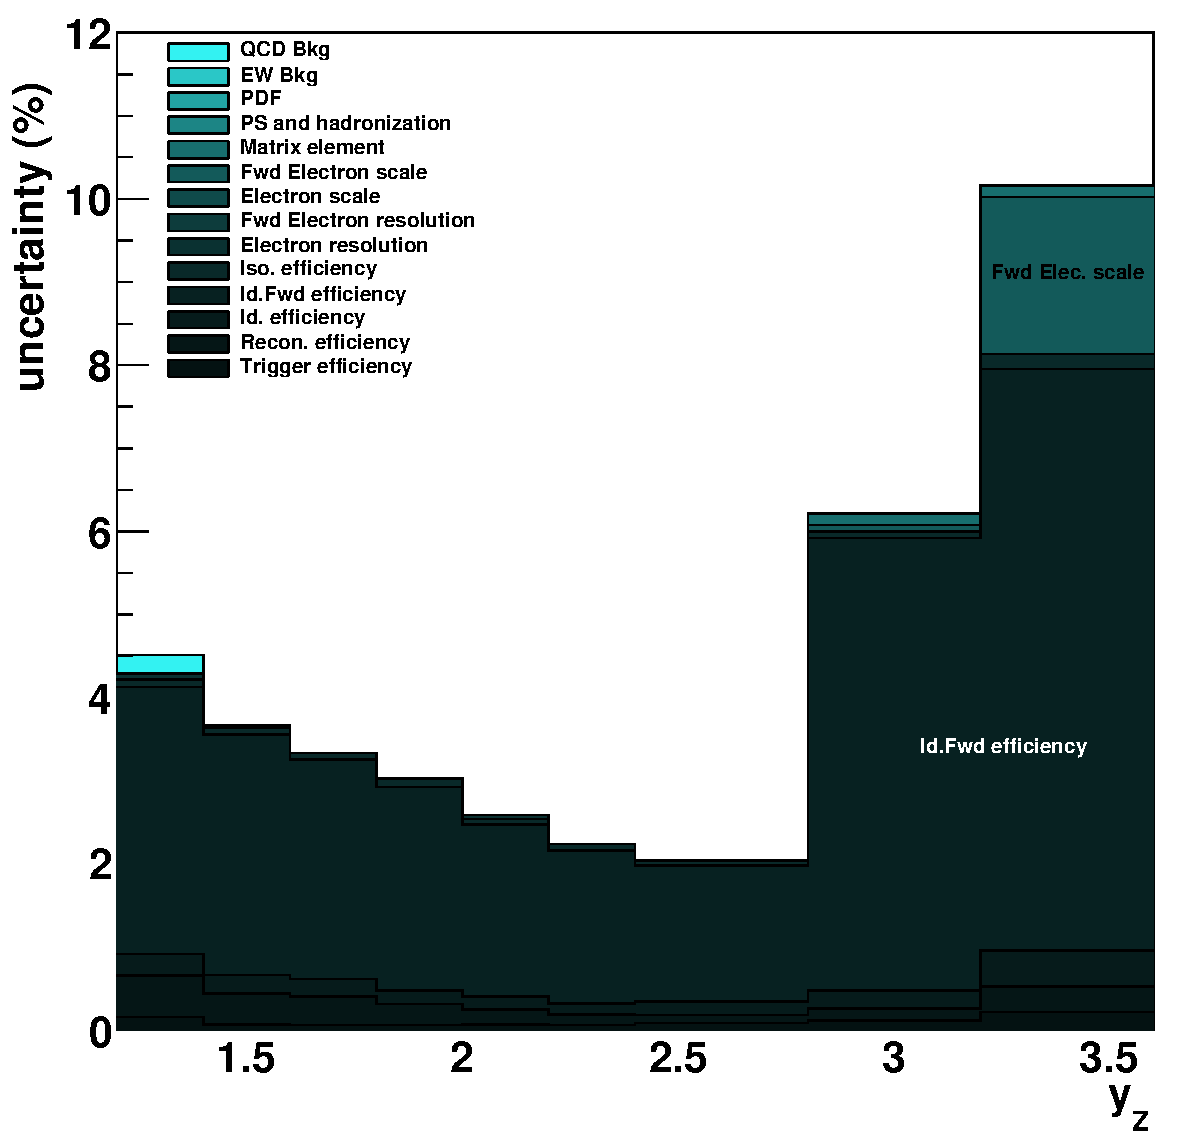
\includegraphics[width=0.48\textwidth]{figures/ZCF_unc_66_116.pdf}
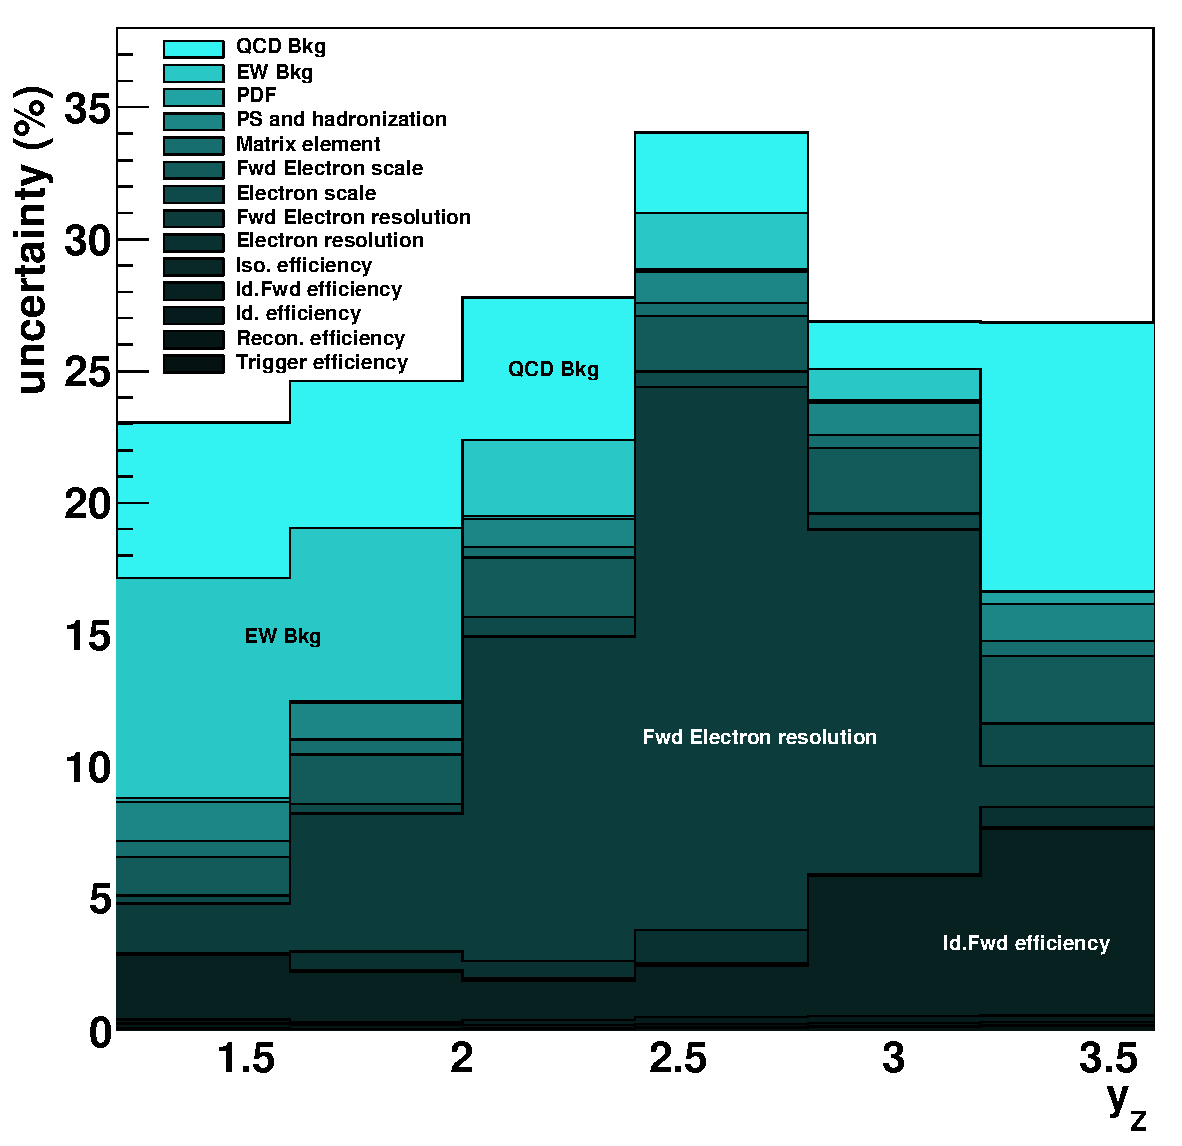
\includegraphics[width=0.48\textwidth]{figures/ZCF_unc_116_150.pdf}
\caption{The list of the systematic uncertainties for the \Zee\ CF analysis for peak mass (left) and high mass (right) regions. The largest sources are explicitly labeled. Each following uncertainty is placed on top of the previous.}
\label{fig:Zee_unc}}
\end{figure}

As the work that was done as part of this thesis contributed to the W,Z inclusive paper~\cite{lib:wz2011} the combined \Zee\ and \Zll\ results were taken from there. The theory comparison that was done for the combined \Zll\ results was outside of the scope of this thesis.

The double-differential analyses were done in the rapidity and mass binning with three mass windows. The \Zee\ central-forward analysis contributed only to two of them: the peak mass ($66 < M_{ee} < 116$~GeV) and the high mass ($116 < M_{ee} < 150$~GeV) windows. Unlike the central-central analysis, the peak mass windows was not divided into additional bins. The analyses results were first calculated in the true experimental fiducial volume, which equals to the experimental phase space and is described in Tab.~\ref{tab:res_phase_space}. Figure~\ref{fig:res_zee_fid} shows the double-differential cross-section with statistical and systematical uncertainties, and Figure~\ref{fig:res_zee_fid_mc} shows the comparison with the different MC simulations. The \Powheg\Pythia\ MC simulation was the one used as signal MC, while the others were used as sources for systematical uncertainties.

\begin{table}
\centering
\begin{tabular}{l l}
\hline \hline
Central electron & $\pt > 23$~GeV, \\
\rule{0pt}{4ex}  & $|\eta| < 2.47$ \\
                 & {\bf excluding} \\
                 & $1.37 < |\eta| < 1.52$ \& $1.6 < |\eta| < 1.7$ \\
\hline
Forward electron & $\pt > 20$~GeV, \\
\rule{0pt}{4ex}  & $2.5 < |\eta| < 4.9$ \\
                 & {\bf excluding} \\
                 & $3.16 < |\eta| < 3.35$ \\
\hline
Mass windows     & $66 < m_{ee} < 116$ \& $116 < m_{ee} < 150$ \\
\hline \hline
\end{tabular}
\caption{The conditions of the experimental phase space.}
\label{tab:res_phase_space}
\end{table}


\begin{figure}
\center{
  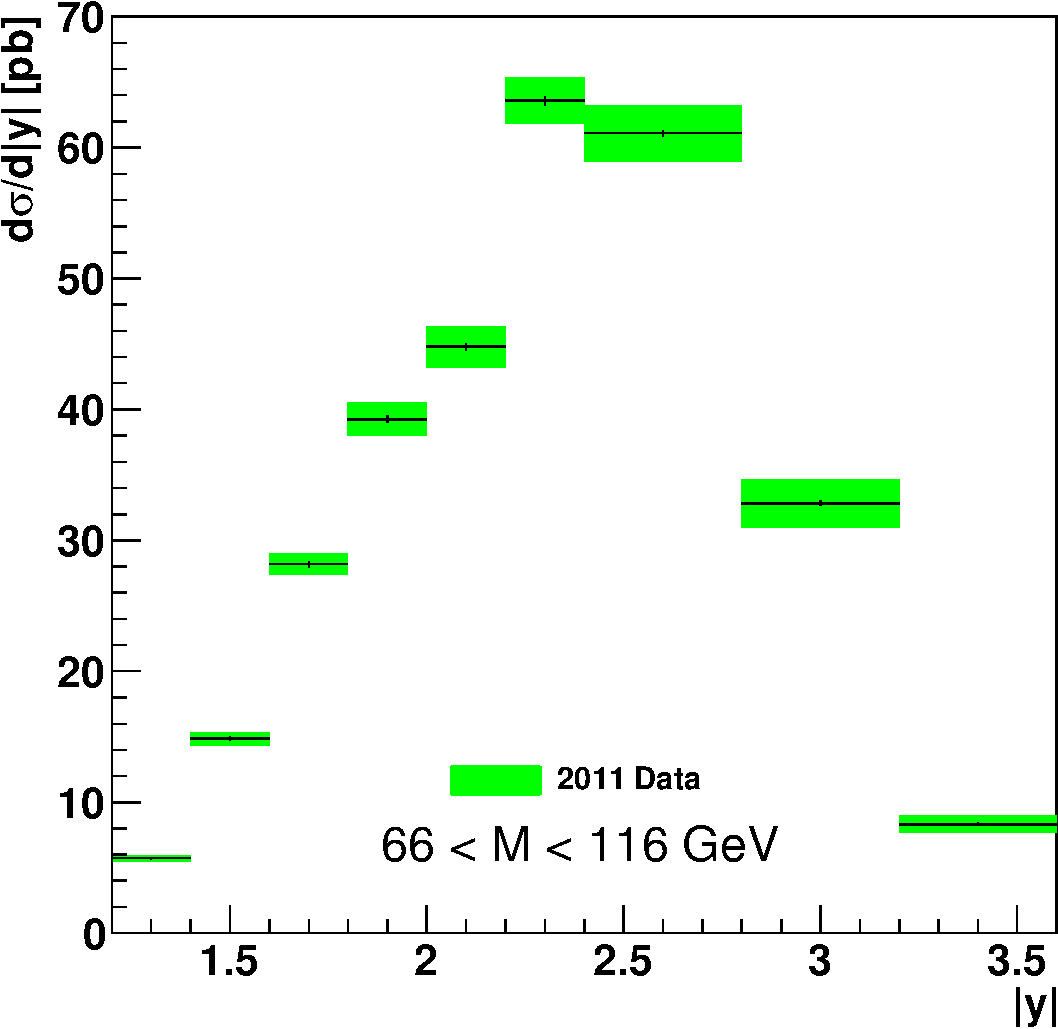
\includegraphics[width=0.45\textwidth]{figures/ZeeCF_Mass_66_116.pdf}
  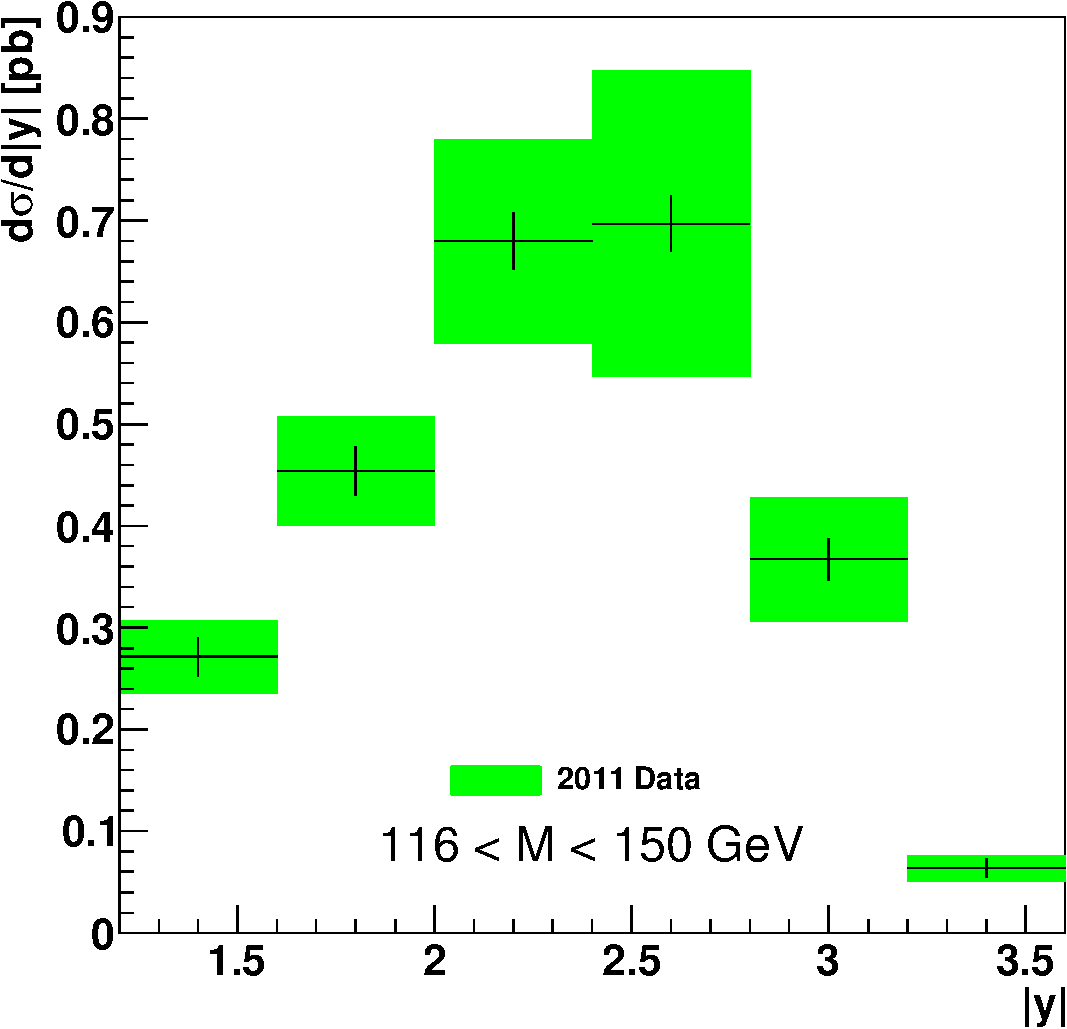
\includegraphics[width=0.45\textwidth]{figures/ZeeCF_Mass_116_150.pdf}
  \caption{\Zee\ CF true experimental fiducial differential cross-section, as a function of absolute boson rapidity for peak mass (left) and high mass (right) regions together with statistical and systematic uncertainties.}
\label{fig:res_zee_fid}}
\end{figure}

\begin{figure}
\center{
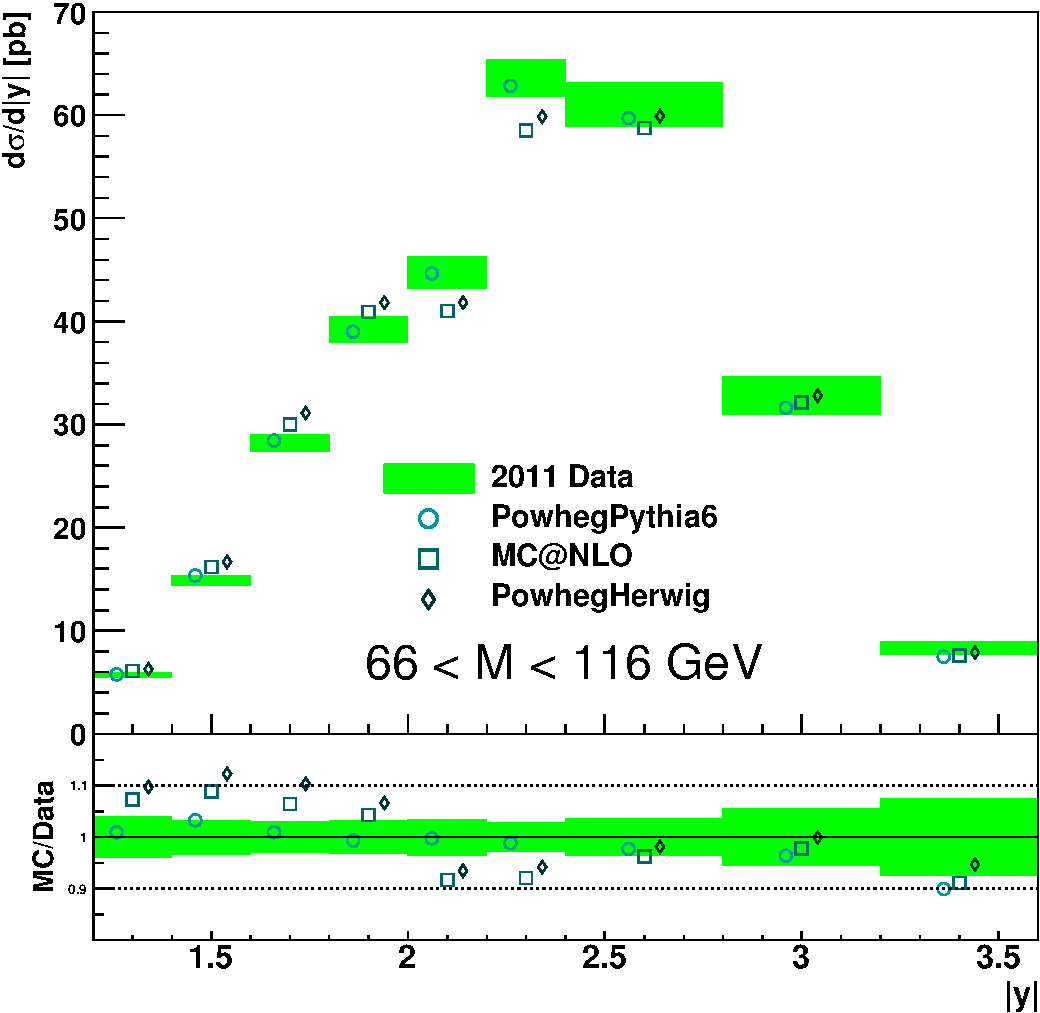
\includegraphics[width=0.45\textwidth]{figures/ZeeCF_Mass_66_116_MC.pdf}
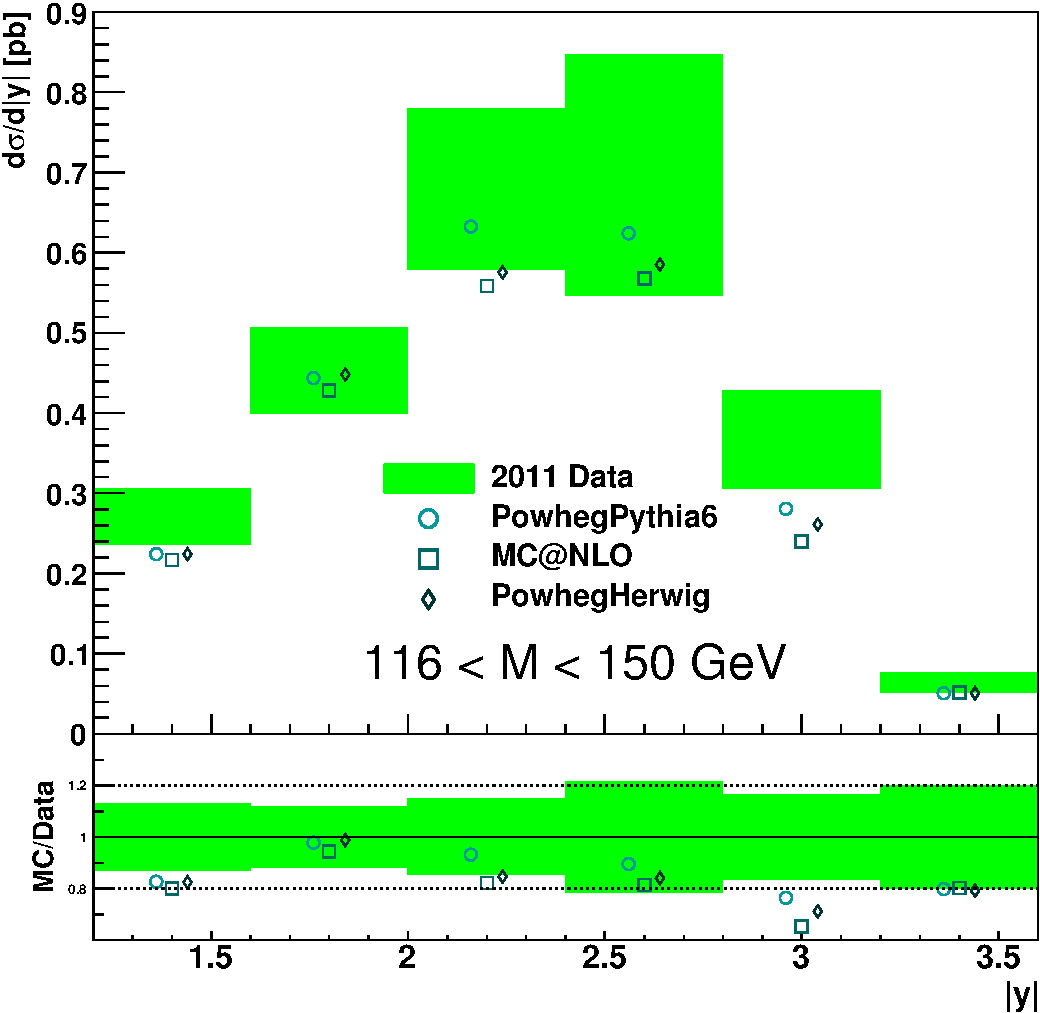
\includegraphics[width=0.45\textwidth]{figures/ZeeCF_Mass_116_150_MC.pdf}
\caption{\Zee\ CF true experimental fiducial differential cross-section, as a function of absolute boson rapidity for peak mass (left) and high mass (right) regions compared to various MC simulations.}
\label{fig:res_zee_fid_mc}}
\end{figure}

The same results in tabular form can be seen in Tabs.~\ref{tab:Zee_NBC_peak} and~\ref{tab:Zee_NBC_high}, where $N$ is the number of events in the bin, $B$ is the estimated number of the background events included in $N$, and $C$ is the true experimental fiducial extrapolation factor, which represents the fraction of all the $Z$ boson that $N$ amounts to.

\begin{table}
\centering
\begin{tabular}{lccc}
\hline \hline
    &   $N$   & $B \pm \delta B$  &  $C \pm \delta C$ \\
\hline
$1.20 < |y| <1.40$          & 4178       & 193.7      $\pm$ 19.7 & 0.381      $\pm$ 0.014 \\
$1.40 < |y| <1.60$          & 12404      & 517.7      $\pm$ 47.4 & 0.436      $\pm$ 0.013 \\
$1.60 < |y| <1.80$          & 24210      & 812.1      $\pm$ 72.7 & 0.453      $\pm$ 0.012 \\
$1.80 < |y| <2.00$          & 33978      & 1021.2     $\pm$ 110.9 & 0.459      $\pm$ 0.014 \\
$2.00 < |y| <2.20$          & 38023      & 1141.2     $\pm$ 123.9 & 0.449      $\pm$ 0.015 \\
$2.20 < |y| <2.40$          & 51372      & 1454.4     $\pm$ 77.6 & 0.429      $\pm$ 0.011 \\
$2.40 < |y| <2.80$          & 101004     & 2613.2     $\pm$ 267.5 & 0.440      $\pm$ 0.015 \\
$2.80 < |y| <3.20$          & 47304      & 1104.4     $\pm$ 52.3 & 0.384      $\pm$ 0.021 \\
$3.20 < |y| <3.60$          & 8453       & 126.6      $\pm$ 29.5 & 0.276      $\pm$ 0.020 \\
\hline \hline
\end{tabular}
\caption{Main components of the differential \Zee\ CF cross-section for peak mass region.}
\label{tab:Zee_NBC_peak}
\end{table}

\begin{table}
\centering
\begin{tabular}{lccc}
\hline \hline
    &   $N$   & $B \pm \delta B$  &  $C \pm \delta C$ \\
\hline
$1.20 < |y| <1.60$          & 1136       & 592.4      $\pm$ 54.8 & 0.552      $\pm$ 0.024 \\
$1.60 < |y| <2.00$          & 1676       & 754.6      $\pm$ 79.2 & 0.565      $\pm$ 0.035 \\
$2.00 < |y| <2.40$          & 2006       & 737.4      $\pm$ 80.2 & 0.531      $\pm$ 0.067 \\
$2.40 < |y| <2.80$          & 1754       & 506.2      $\pm$ 48.6 & 0.515      $\pm$ 0.107 \\
$2.80 < |y| <3.20$          & 659        & 120.7      $\pm$ 12.8 & 0.439      $\pm$ 0.068 \\
$3.20 < |y| <3.60$          & 84         & 15.2       $\pm$ 8.3 & 0.348      $\pm$ 0.031 \\
\hline \hline
\end{tabular}
\caption{Main components of the differential \Zee\ CF cross-section for high mass region.}
\label{tab:Zee_NBC_high}
\end{table}

In Tabs.~\ref{tab:Zee_peak} and~\ref{tab:Zee_high} the results of the cross-section as measured in the true experimental fiducial volume can be found along with statistical, systematical and luminosity uncertainties.

\begin{table}
\centering
\begin{tabular}{lc}
\hline \hline
$1.20 < |y| <1.40$          & 5.715 $\pm$ 0.101 (stat) $\pm$ 0.207 (syst) $\pm$ 0.103 (lum) [pb]  \\
$1.40 < |y| <1.60$          & 14.864 $\pm$ 0.151 (stat) $\pm$ 0.465 (syst) $\pm$ 0.268 (lum) [pb]  \\
$1.60 < |y| <1.80$          & 28.200 $\pm$ 0.206 (stat) $\pm$ 0.792 (syst) $\pm$ 0.508 (lum) [pb]  \\
$1.80 < |y| <2.00$          & 39.245 $\pm$ 0.233 (stat) $\pm$ 1.214 (syst) $\pm$ 0.706 (lum) [pb]  \\
$2.00 < |y| <2.20$          & 44.786 $\pm$ 0.260 (stat) $\pm$ 1.534 (syst) $\pm$ 0.806 (lum) [pb]  \\
$2.20 < |y| <2.40$          & 63.598 $\pm$ 0.317 (stat) $\pm$ 1.717 (syst) $\pm$ 1.145 (lum) [pb]  \\
$2.40 < |y| <2.80$          & 61.087 $\pm$ 0.207 (stat) $\pm$ 2.126 (syst) $\pm$ 1.100 (lum) [pb]  \\
$2.80 < |y| <3.20$          & 32.826 $\pm$ 0.162 (stat) $\pm$ 1.811 (syst) $\pm$ 0.591 (lum) [pb]  \\
$3.20 < |y| <3.60$          & 8.313 $\pm$ 0.102 (stat) $\pm$ 0.614 (syst) $\pm$ 0.150 (lum) [pb]  \\
\hline \hline
\end{tabular}
\caption{Differential \Zee\ CF cross-section for the peak mass region, measured in the true experimental fiducial volume together with uncertainties.}
\label{tab:Zee_peak}
\end{table}

\begin{table}
\centering
\begin{tabular}{lc}
\hline \hline
$1.20 < |y| <1.60$          & 0.271 $\pm$ 0.018 (stat) $\pm$ 0.030 (syst) $\pm$ 0.005 (lum) [pb]  \\
$1.60 < |y| <2.00$          & 0.454 $\pm$ 0.023 (stat) $\pm$ 0.047 (syst) $\pm$ 0.008 (lum) [pb]  \\
$2.00 < |y| <2.40$          & 0.680 $\pm$ 0.027 (stat) $\pm$ 0.095 (syst) $\pm$ 0.012 (lum) [pb]  \\
$2.40 < |y| <2.80$          & 0.697 $\pm$ 0.027 (stat) $\pm$ 0.147 (syst) $\pm$ 0.013 (lum) [pb]  \\
$2.80 < |y| <3.20$          & 0.367 $\pm$ 0.019 (stat) $\pm$ 0.057 (syst) $\pm$ 0.007 (lum) [pb]  \\
$3.20 < |y| <3.60$          & 0.064 $\pm$ 0.009 (stat) $\pm$ 0.009 (syst) $\pm$ 0.001 (lum) [pb]  \\
\hline \hline
\end{tabular}
\caption{Differential \Zee\ CF cross-section for the high mass region, measured in the true experimental fiducial volume together with uncertainties.}
\label{tab:Zee_high}
\end{table}

For the comparison with the theoretical predictions, the results were extrapolated to the fiducial volume, which differs from the true experimental fiducial volume in inclusion of the crack regions. As a result, the values are about $\sim$20\% higher as in the true experimental one. The theoretical predictions were calculated at NLO using the MCFM software~\cite{lib:res_MCFM} and then corrected to NNLO using the k-factor produces by FEWZ software~\cite{lib:res_FEWZ1, lib:res_FEWZ2}. Figure~\ref{fig:res_zee_fid_th} shows the comparison to the theoretical predictions done with various PDF sets.

\begin{figure}
\center{
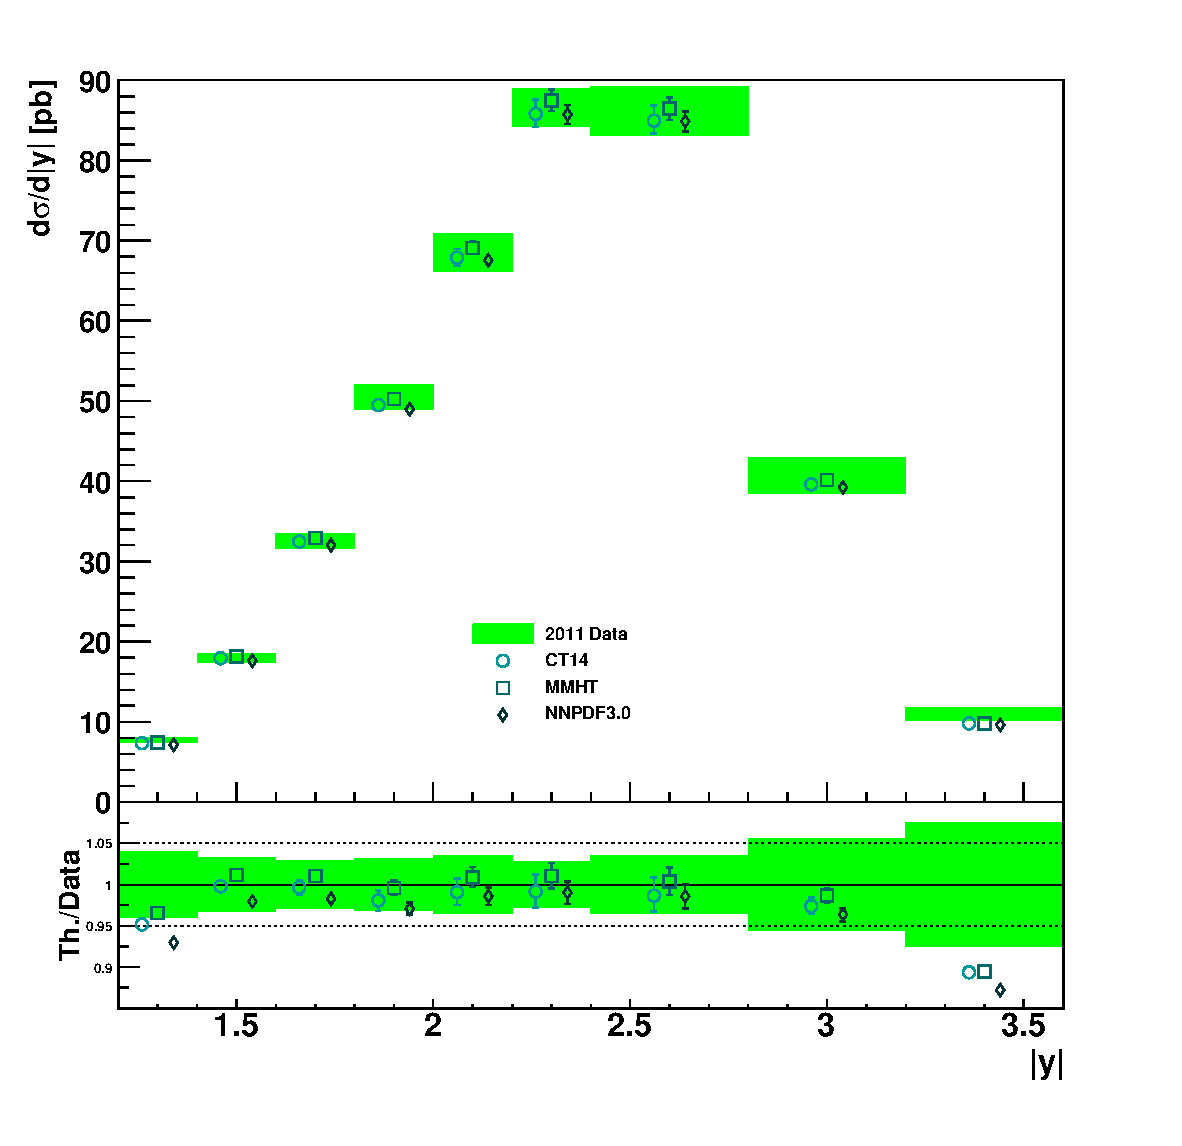
\includegraphics[width=0.45\textwidth]{figures/ZeeCF_Mass_66_116_th.pdf}
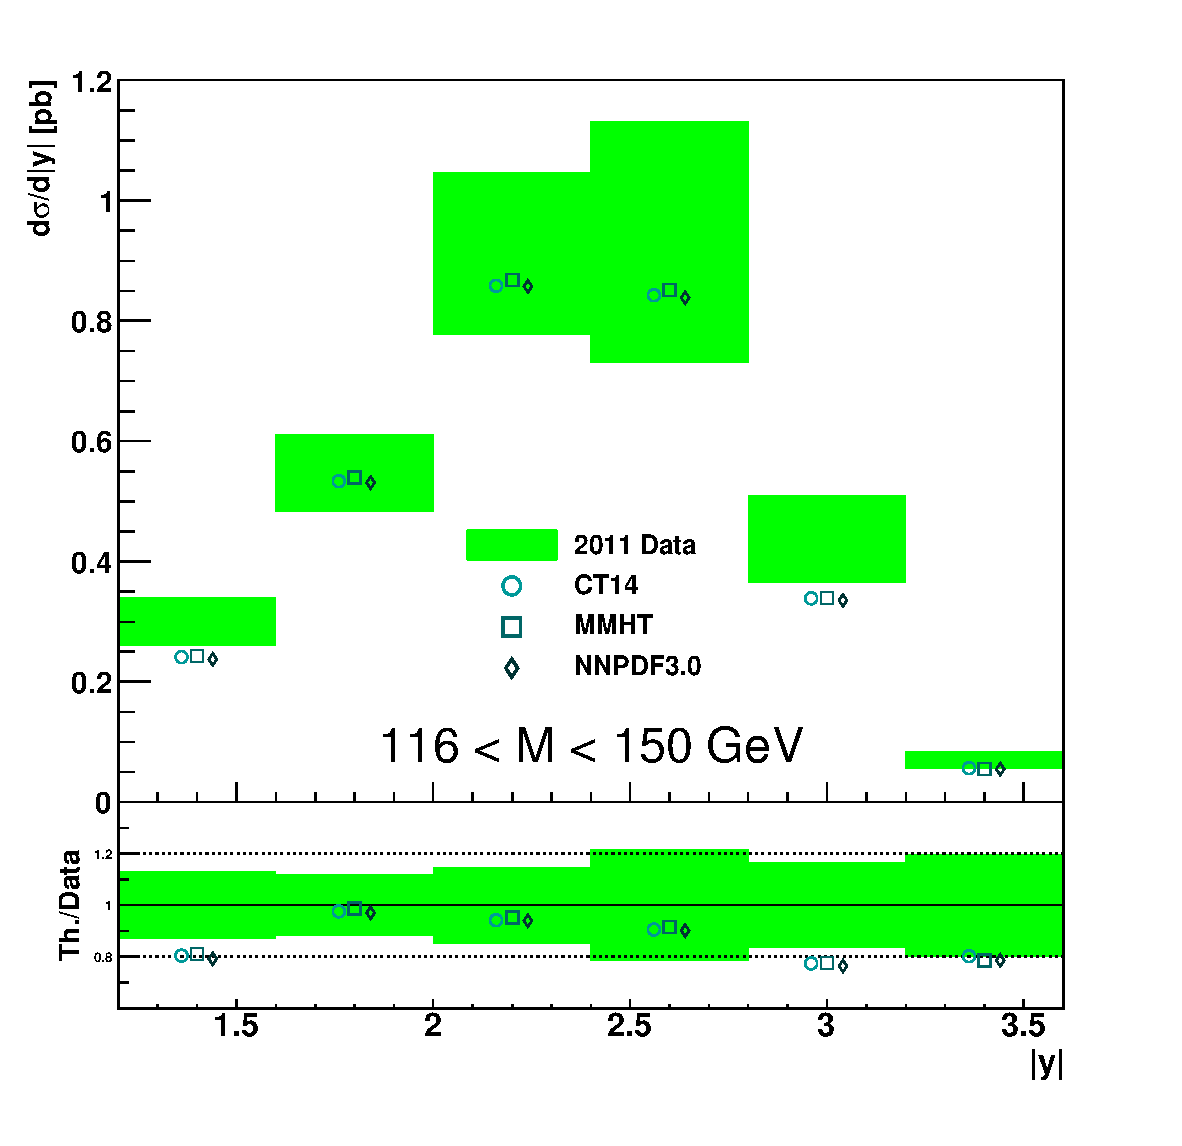
\includegraphics[width=0.45\textwidth]{figures/ZeeCF_Mass_116_150_th.pdf}
\caption{\Zee\ CF extrapolated fiducial cross-section, as a function of absolute boson rapidity for peak mass (left) and high mass (right) regions compared to various theoretical predictions.}
\label{fig:res_zee_fid_th}}
\end{figure}

The following results for the \Zll\ combined cross sections were taken from the W,Z inclusive paper~\cite{lib:wz2011}, as the combination of the results was outside of the scope of this thesis. The combination technique was described in Section~\ref{sec:ZeeCS_comb}. It is important to note, that \Zee\ central-forward data contributed only to the $|y| > 1.2$ part of the combined cross-section, and the last three bins $|y| > 2.4$ of it can be seen as purely \Zee\ central-forward. The combined cross-section itself can be seen in Figure~\ref{fig:Zll}, while the comparison with the different theoretical predictions can be seen in Figure~\ref{fig:Zll_theory}.

\begin{figure}
\center{
  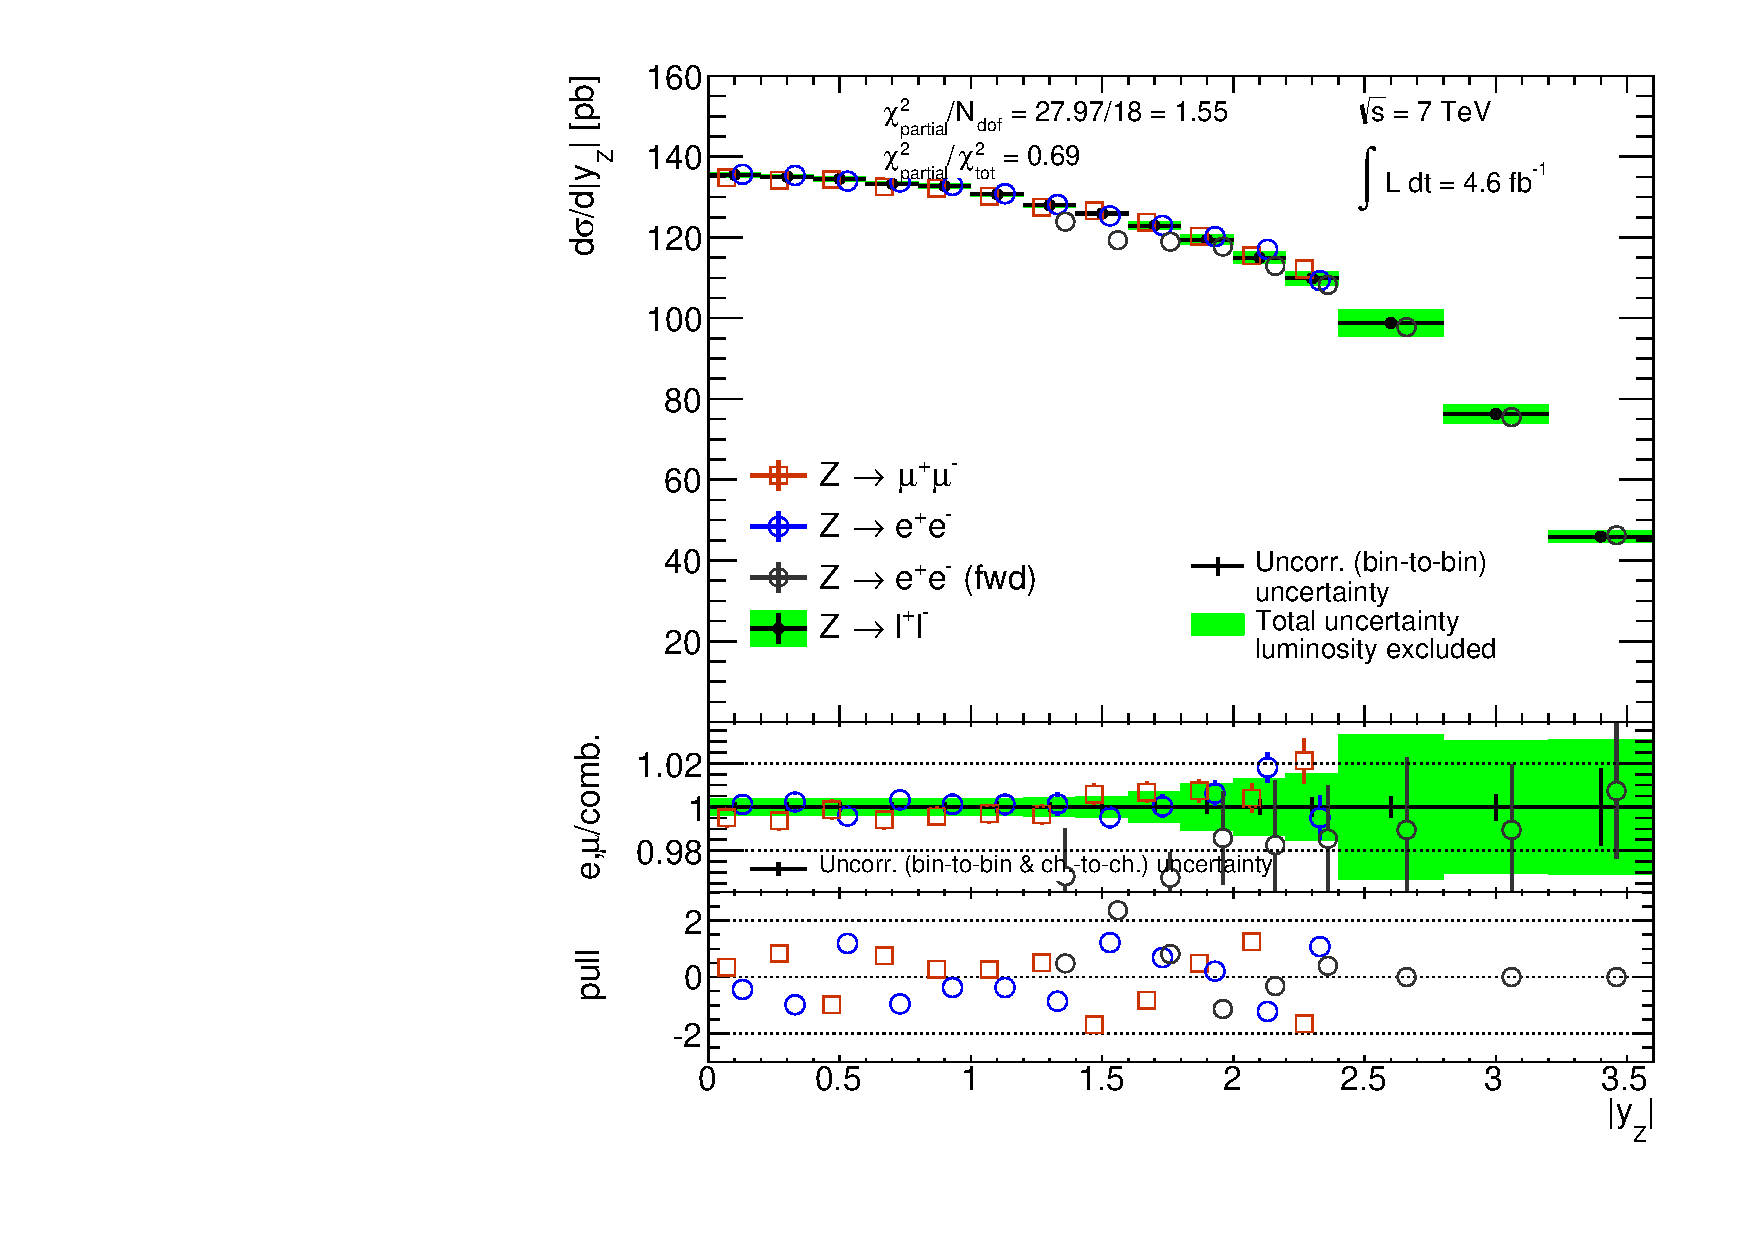
\includegraphics[width=0.45\textwidth]{figures/Z_66_116_combined.pdf}
  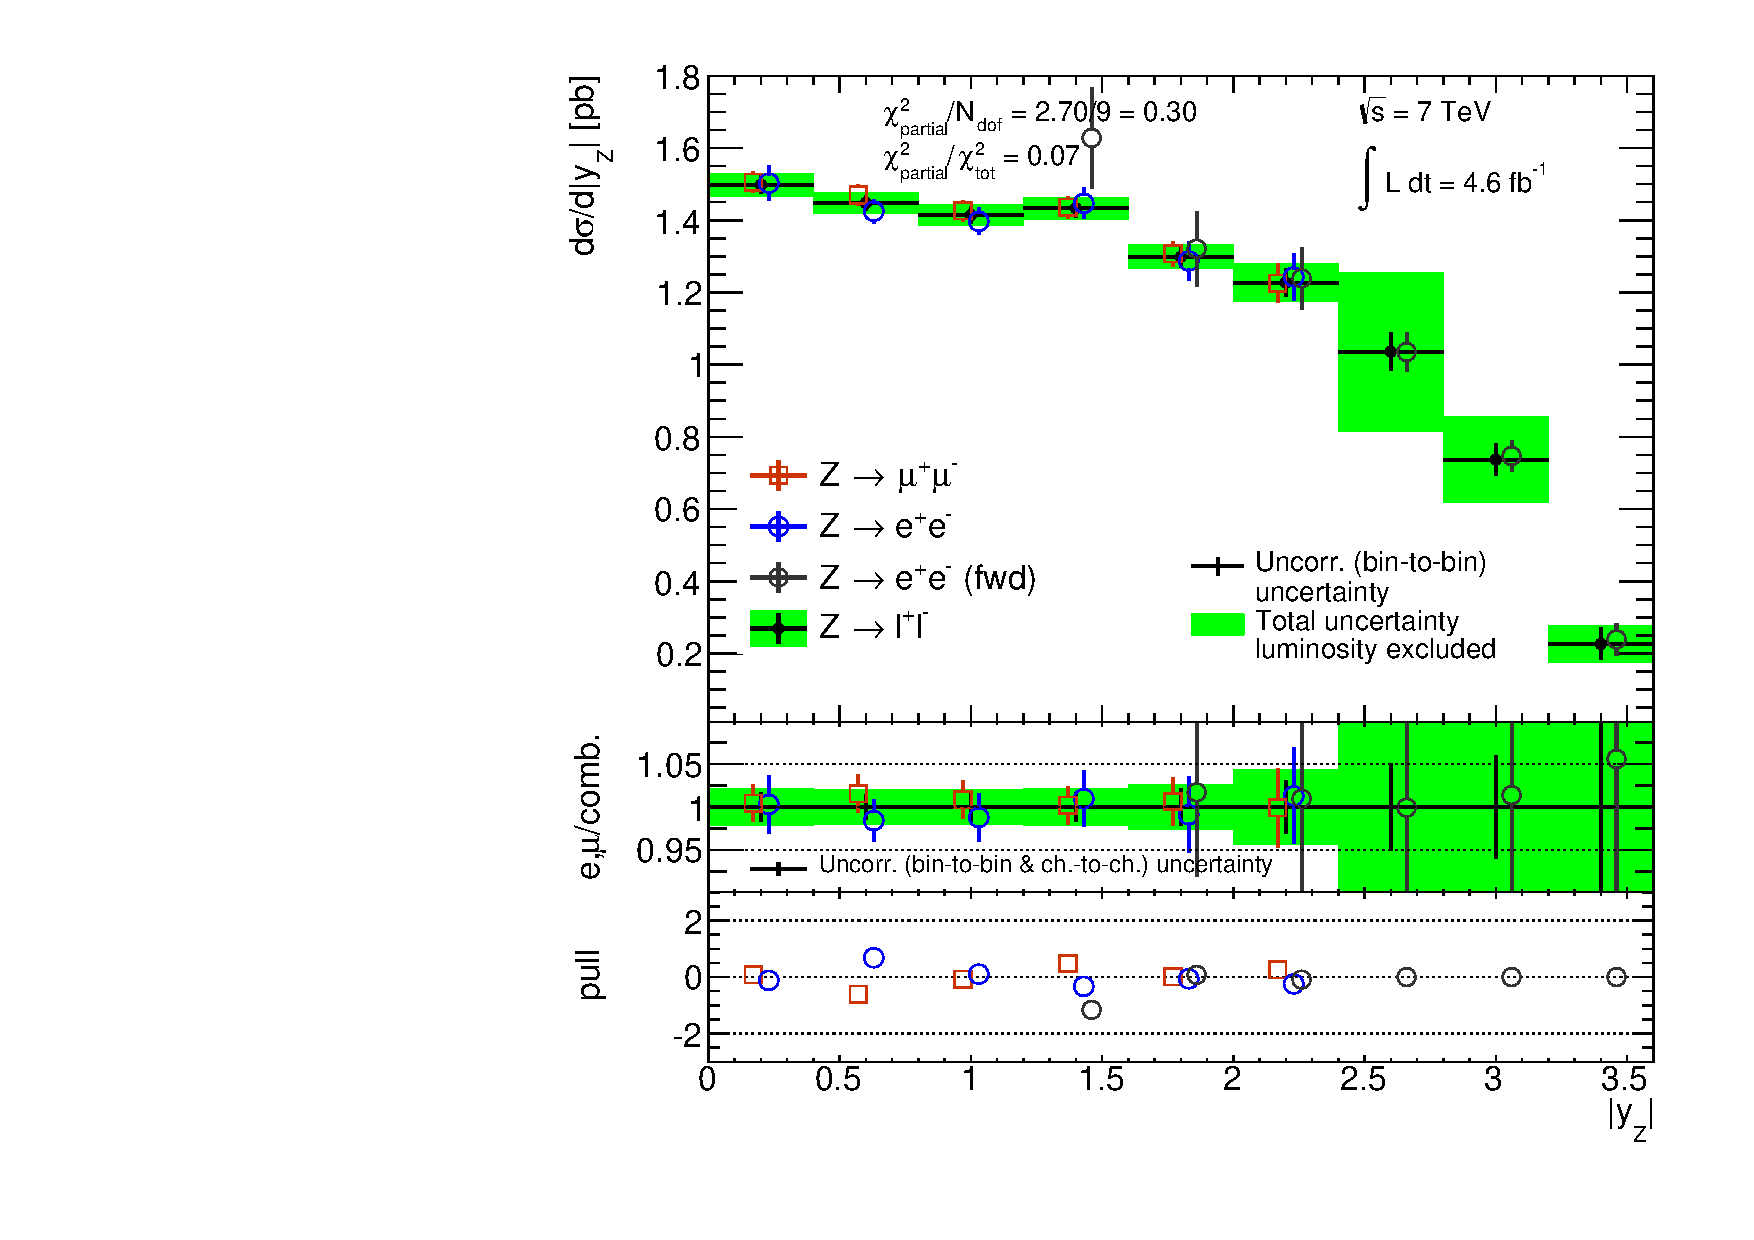
\includegraphics[width=0.45\textwidth]{figures/Z_116_150_combined.pdf}
  \caption{Combined \Zll\ cross-section for peak mass (left) and high mass (right) regions together with uncertainties. The ratio and the pull values are also shown for each source.~\cite{lib:wz2011}}
\label{fig:Zll}}
\end{figure}

\begin{figure}
\center{
  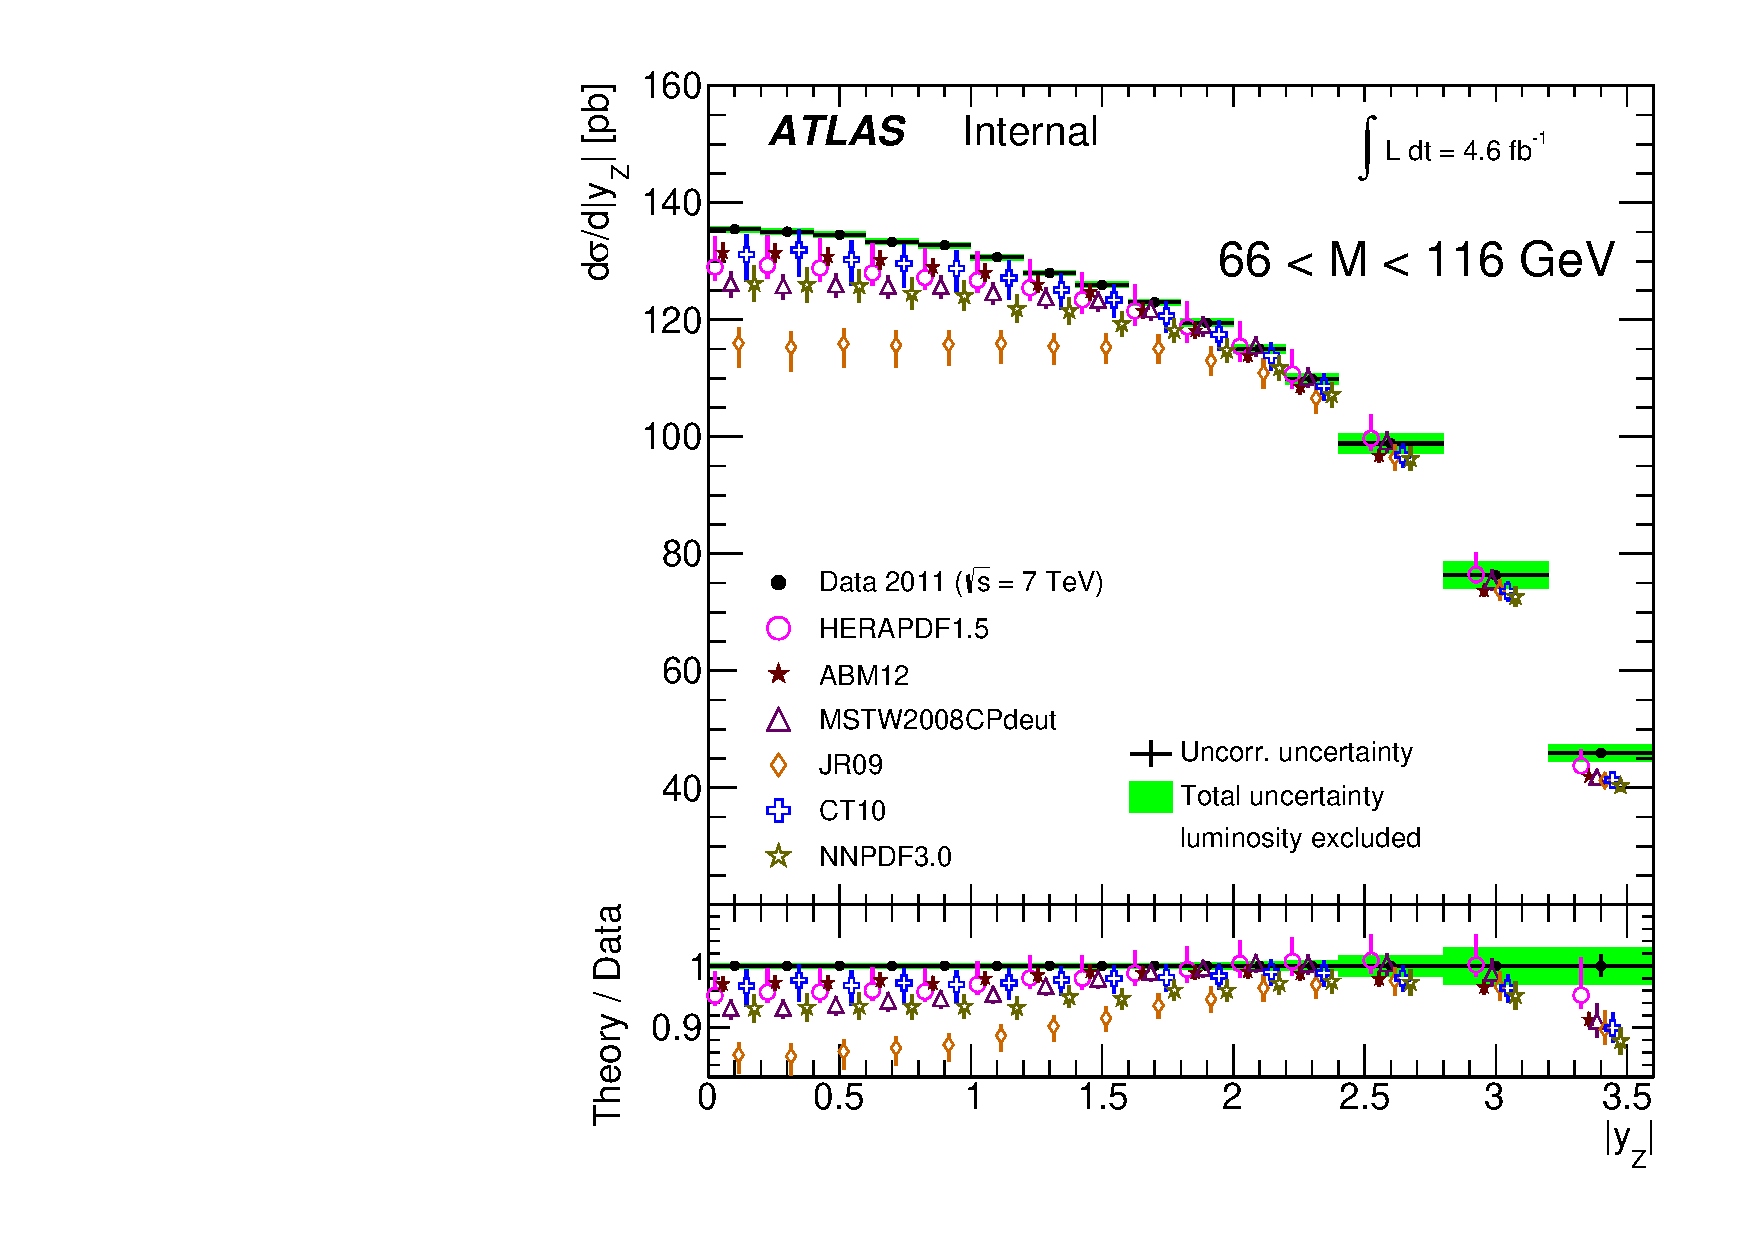
\includegraphics[width=0.45\textwidth]{figures/Z_66_116_NNLO_combined.pdf}
  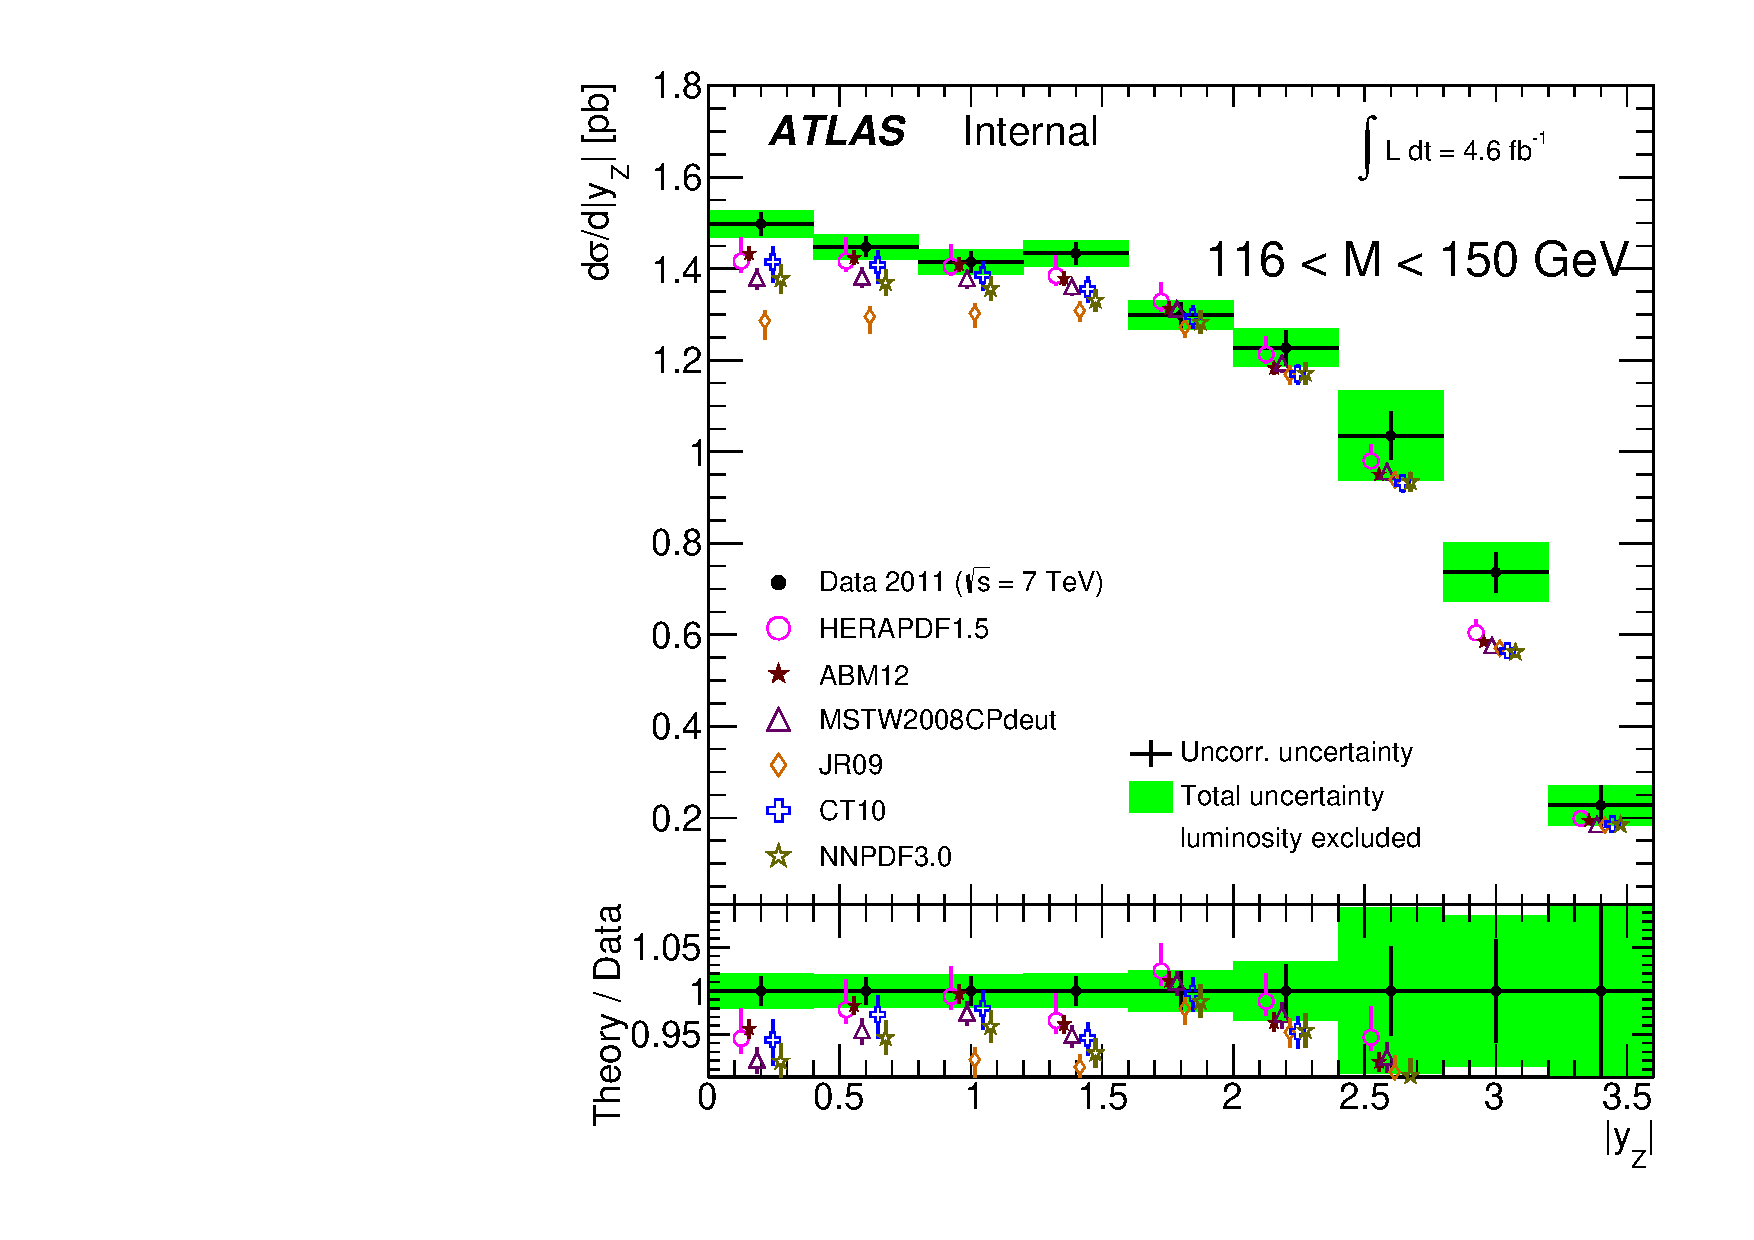
\includegraphics[width=0.45\textwidth]{figures/Z_116_150_NNLO_combined.pdf}
  \caption{Comparison of the combined \Zll\ cross-section with NNLO predictions using various PDF sets for peak mass (left) and high mass (right) regions together with uncertainties. The ratios are also shown.~\cite{lib:wz2011}}
\label{fig:Zll_theory}}
\end{figure}
